\documentclass[12pt,b5paper]{ltjsarticle}

%\usepackage[margin=15truemm, top=5truemm, bottom=5truemm]{geometry}
%\usepackage[margin=10truemm,left=15truemm]{geometry}
\usepackage[margin=10truemm]{geometry}

\usepackage{amsmath,amssymb}
%\pagestyle{headings}
\pagestyle{empty}

%\usepackage{listings,url}
%\renewcommand{\theenumi}{(\arabic{enumi})}

\usepackage{graphicx}

%\usepackage{tikz}
%\usetikzlibrary {arrows.meta}
%\usepackage{wrapfig}	% required for `\wrapfigure' (yatex added)
%\usepackage{bm}	% required for `\bm' (yatex added)

% ルビを振る
%\usepackage{luatexja-ruby}	% required for `\ruby'

%% 核Ker 像Im Hom を定義
%\newcommand{\Img}{\mathop{\mathrm{Im}}\nolimits}
%\newcommand{\Ker}{\mathop{\mathrm{Ker}}\nolimits}
%\newcommand{\Hom}{\mathop{\mathrm{Hom}}\nolimits}

%\DeclareMathOperator{\Rot}{rot}
%\DeclareMathOperator{\Div}{div}
%\DeclareMathOperator{\Grad}{grad}
%\DeclareMathOperator{\arcsinh}{arcsinh}
%\DeclareMathOperator{\arccosh}{arccosh}
%\DeclareMathOperator{\arctanh}{arctanh}



%\usepackage{listings,url}
%
%\lstset{
%%プログラム言語(複数の言語に対応,C,C++も可)
%  language = Python,
%%  language = Lisp,
%%  language = C,
%  %背景色と透過度
%  %backgroundcolor={\color[gray]{.90}},
%  %枠外に行った時の自動改行
%  breaklines = true,
%  %自動改行後のインデント量(デフォルトでは20[pt])
%  breakindent = 10pt,
%  %標準の書体
%%  basicstyle = \ttfamily\scriptsize,
%  basicstyle = \ttfamily,
%  %コメントの書体
%%  commentstyle = {\itshape \color[cmyk]{1,0.4,1,0}},
%  %関数名等の色の設定
%  classoffset = 0,
%  %キーワード(int, ifなど)の書体
%%  keywordstyle = {\bfseries \color[cmyk]{0,1,0,0}},
%  %表示する文字の書体
%  %stringstyle = {\ttfamily \color[rgb]{0,0,1}},
%  %枠 "t"は上に線を記載, "T"は上に二重線を記載
%  %他オプション:leftline,topline,bottomline,lines,single,shadowbox
%  frame = TBrl,
%  %frameまでの間隔(行番号とプログラムの間)
%  framesep = 5pt,
%  %行番号の位置
%  numbers = left,
%  %行番号の間隔
%  stepnumber = 1,
%  %行番号の書体
%%  numberstyle = \tiny,
%  %タブの大きさ
%  tabsize = 4,
%  %キャプションの場所("tb"ならば上下両方に記載)
%  captionpos = t
%}



\begin{document}

\hrulefill

$0< \alpha < 1$を実定数とするとき、
留数定理を用いて以下を示せ。
\begin{equation}
 \int_{-\infty}^{\infty} \frac{e^{\alpha x}}{e^{x}+1}dx
  = \frac{\pi}{\sin{(\alpha\pi)}}
\end{equation}

\dotfill


$f(x)=\frac{e^{\alpha x}}{e^{x}+1}$とする。
$f(x)$は実数上正則だが、
複素数上の関数$f(z)$として考えると極を持つ。

$e^{z}+1=0$を満たすのは$z=\pi i$のみである。
$e^{z}$をTaylor展開すると次のようになる。
\begin{equation}
 e^{z}=\sum_{n=0}^{\infty}\frac{z^n}{n!}
  = 1 + z + \frac{1}{2}z^{2} + \frac{1}{6}z^{3} + \cdots
\end{equation}

ここで、Taylor展開の$z$を$z-\pi i$に置き換えると次のようになる。
\begin{align}
 e^{z} =& e^{z-\pi i + \pi i}
  = e^{z-\pi i} e^{\pi i}\\
 =& e^{\pi i} \sum_{n=0}^{\infty}\frac{(z-\pi i)^n}{n!}
 = -\left( 1 + (z-\pi i) + \frac{1}{2}(z-\pi i)^{2} + \frac{1}{6}(z-\pi i)^{3} + \cdots \right)
\end{align}

$e^z+1$は上の式に1を加えるので定数項が消え、
最低次数の項が$-(z-\pi i)$となる。

つまり、
$f(z)=\frac{e^{\alpha z}}{e^{z}+1}$は
$z=\pi i$について1位の極を持つ。

そこで留数$Res(f,\pi i)$を計算する。
\begin{equation}
 Res(f,\pi i)
 = \lim_{z\to \pi i}(z-\pi i) \frac{e^{\alpha z}}{e^{z}+1}\\
 = \frac{e^{\alpha \pi i}}{e^{\pi i}}
  = -e^{\alpha \pi i}
  \label{res_value}
\end{equation}

積分路を複素平面上に長方形を作り
その周りを反時計回りの周回で考える。

実数$a > 0$を決める。
長方形の4辺を次のように決める。
\begin{itemize}
 \item [$L_1$]
       $-a$から$a$までの直線
 \item [$L_2$]
       $a$から$a+2\pi i$までの直線
 \item [$L_3$]
       $a+2\pi i$から$-a+2\pi i$までの直線
 \item [$L_2$]
       $-a+2\pi i$から$-a$までの直線
\end{itemize}
これらをまとめて
$\Gamma = L_1 + L_2 + L_3 + L_4$
とする。

%%%
%%% 図
%%%
%\begin{figure}
%\label{fig:hoge}
\centerline{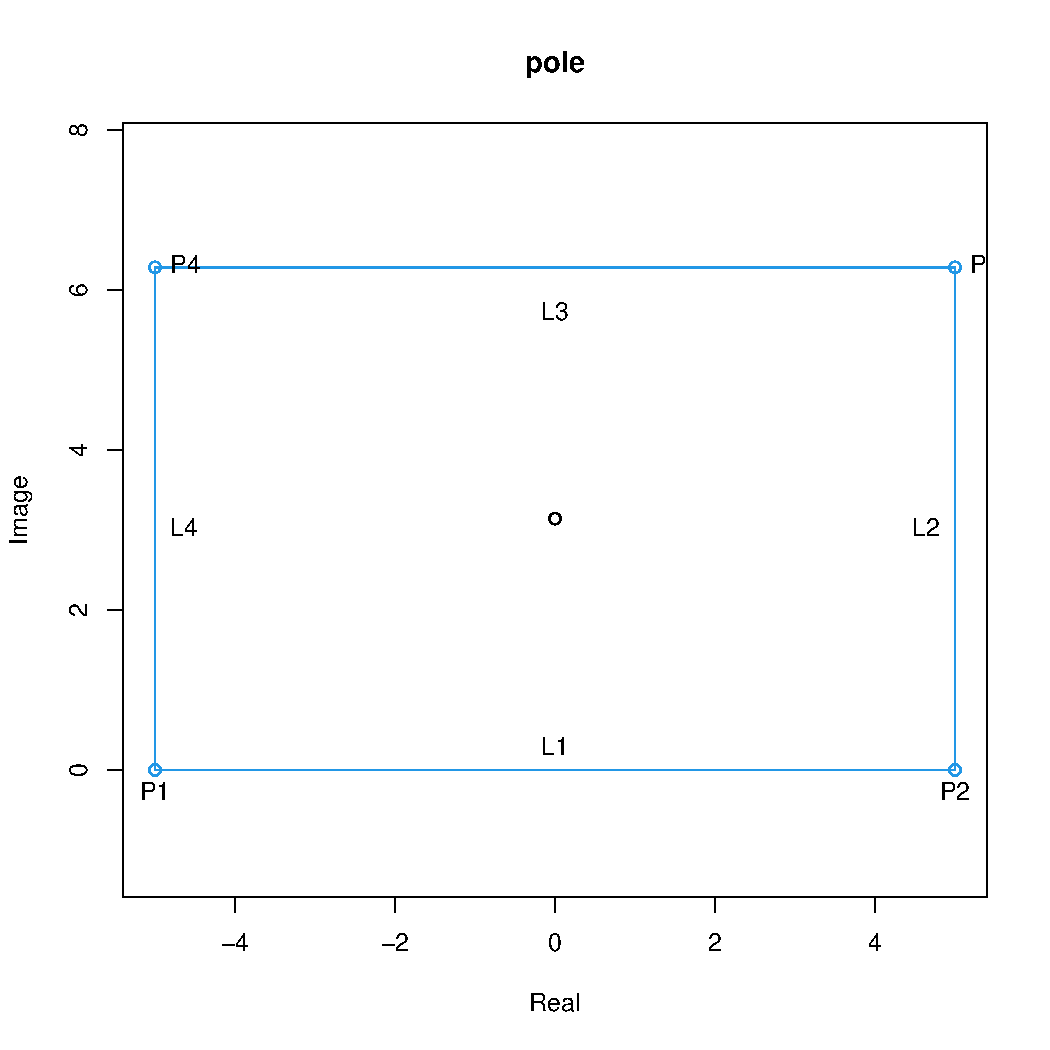
\includegraphics[width=0.5\textwidth]{pole_plot_R.pdf}}
%\caption{極の場所と積分路}
%\end{figure}

積分は次のように分けられる。
\begin{equation}
 \int_{\Gamma} f(z) dz
  =\int_{L_1} f(z) dz + \int_{L_2} f(z) dz
  +\int_{L_3} f(z) dz + \int_{L_4} f(z) dz
\end{equation}

$L_1$上の積分は次のように実数上の積分である。
\begin{equation}
 \int_{L_1} f(z) dz = \int_{-a}^{a} f(x) dx
\end{equation}

$L_2$上の積分は
$a$から$a+2\pi i$までの線分上で行う。
$z=a+yi$として
$y : 0\to2\pi$の範囲で積分する。
このとき、$dz=i dy$である。
\begin{align}
 \int_{L_2} f(z) dz
  =& \int_{L_2} \frac{e^{\alpha z}}{e^{z}+1} dz
  = \int_{0}^{2\pi}
  \frac{e^{\alpha (a+yi)}}{e^{a+yi}+1}
  i dy\\
  =& \int_{0}^{2\pi}
  \frac{ e^{\alpha a} e^{\alpha yi} }{ e^{a}(e^{yi} +e^{-a}) }
  i dy
  = \int_{0}^{2\pi}
  \frac{ e^{\alpha yi}\ i }{ e^{(1-\alpha)a}(e^{yi} +e^{-a}) }
  dy
\end{align}

\begin{align}
 \left\lvert \int_{L_2} f(z) dz \right\rvert
 \leq &  \int_{0}^{2\pi} \left\lvert
 \frac{ e^{\alpha yi}\ i }{ e^{(1-\alpha)a}(e^{yi} +e^{-a}) }
 \right\rvert dy
 \leq \int_{0}^{2\pi}
 \frac{ \lvert e^{\alpha yi} \rvert \lvert i \rvert}{ \lvert e^{(1-\alpha)a} \rvert \lvert e^{yi} +e^{-a} \rvert }
 dy
\end{align}

ここで、$e^{i\theta}$は単位円周上の複素数を表すので、
$\lvert e^{\alpha yi} \rvert =1$である。
$e^{yi}$は単位円周上の複素数であり、
$e^{-a}$は$0<e^{-a}<1$となる実数である。
よって、
$\lvert e^{yi} +e^{-a} \rvert \geq \lvert -1 + e^{-a} \rvert =1-e^{-a}$
である。
これにより上の不等式は次のようになる。
\begin{align}
 \left\lvert \int_{L_2} f(z) dz \right\rvert
  \leq & \int_{0}^{2\pi}
 \frac{ \lvert e^{\alpha yi} \rvert \lvert i \rvert}{ \lvert e^{(1-\alpha)a} \rvert \lvert e^{yi} +e^{-a} \rvert }
 dy\\
 \leq & \int_{0}^{2\pi}
 \frac{1}{ e^{(1-\alpha)a}(1 -e^{-a}) }dy
 = \frac{2\pi}{ e^{(1-\alpha)a}(1 -e^{-a}) }
 \to 0 \ (a\to\infty)
\end{align}

つまり、$L_2$上の積分は0になることがわかる。


$L_3$上の積分は
$a+2\pi i$から$-a+2\pi i$までの線分上で行う。
$z=x+2\pi i$として、$x:a\to -a$の範囲で積分する。
この時、$dz=dx$である。
\begin{align}
 \int_{L_3} f(z) dz
  =& \int_{L_3} \frac{e^{\alpha z}}{e^{z}+1} dz
  = \int_{a}^{-a}
  \frac{e^{\alpha (x+2\pi i)}}{e^{x+2\pi i}+1}
  dx\\
  =& \int_{a}^{-a}
  \frac{ e^{\alpha x} e^{2 \alpha \pi i} }{ e^{x} e^{2\pi i} +1}
  dx
  = e^{2 \alpha \pi i}
 \int_{a}^{-a} \frac{ e^{\alpha x}}{ e^{x} +1} dx
\end{align}


最後に$L_4$上の積分を考える。
$-a+2\pi i$から$-a$までの線分上での積分で
$z=-a+yi$として、$y:2\pi\to 0$の範囲で行う。
$dz=idy$である。
\begin{equation}
 \int_{L_4} f(z) dz
  = \int_{L_4} \frac{e^{\alpha z}}{e^{z}+1} dz
  = \int_{2\pi}^{0}
  \frac{e^{\alpha (-a+yi)}}{e^{-a+yi}+1}
  i dy
  = \int_{0}^{2\pi}
  \frac{ - e^{\alpha yi} i}{ e^{\alpha a} (e^{-a}e^{yi} + 1) }
  dy
\end{equation}

$L_2$の時と同じように不等式を考える。
\begin{align}
 \left\lvert \int_{L_4} f(z) dz \right\rvert
 \leq &
 \int_{0}^{2\pi}
  \frac{ \lvert - e^{\alpha yi} i \rvert }{ e^{\alpha a} \lvert e^{-a}e^{yi} + 1 \rvert }
  dy
 \leq \int_{0}^{2\pi} \frac{ 1 }{ e^{\alpha a} (1- e^{-a}) } dy\\
 =&  \frac{ 2\pi }{ e^{\alpha a} (1- e^{-a}) }
 \to 0 \ (a\to\infty)
\end{align}
上記の$\lvert e^{-a}e^{yi} + 1 \rvert$は
$1$を中心とした半径$e^{-a}$の円周上の点の大きさを表している。
$a$は正の実数であるので、$e^{-a}<1$となることから
$\lvert e^{-a}e^{yi} + 1 \rvert \geq 1-e^{-a}$となる。

これにより$L_4$上の積分も0となる。

この為、$\Gamma$上の積分は次のようになる。
\begin{equation}
 \lim_{a\to\infty} \int_{\Gamma} f(z) dz
  = \int_{-\infty}^{\infty} f(x) dx
  + e^{2 \alpha \pi i}
 \int_{\infty}^{-\infty}
 %\frac{ e^{\alpha x}}{ e^{x} +1}
 f(x) dx
 = (1-e^{2 \alpha \pi i})\int_{-\infty}^{\infty} f(x) dx
\end{equation}

留数の計算結果(\ref{res_value})より
$\Gamma$上の積分は次のようになる。
\begin{equation}
 \int_{\Gamma} f(z) dz
  =
 2\pi i ( -e^{\alpha \pi i} )
\end{equation}

このことから次の式が得られる。
\begin{align}
 \int_{-\infty}^{\infty} f(x) dx
  =&
  \frac{ 2\pi i ( -e^{\alpha \pi i} ) }{ 1-e^{2 \alpha \pi i} }
  = \frac{ -2\pi i }{ e^{-\alpha \pi i}-e^{ \alpha \pi i} }\\
  =& \frac{ -2\pi i }{ (\cos{(-\alpha \pi)}+i\sin{(-\alpha \pi)})-(\cos{(\alpha \pi)}+i\sin{(\alpha \pi)}) }\\
 =& \frac{ -2\pi i }{ -i\sin{(\alpha \pi)}-i\sin{(\alpha \pi)} }
  = \frac{\pi}{\sin{(\alpha \pi)}}
\end{align}


\hrulefill

\end{document}
